%!TEX root = ../../secondYearReport.tex

Continuing the activities which started in the first year of the project, IIT further improved the torque whole-body controller. During the second year of the project, attention was mainly on rigid contacts even if the theoretical and software development was guided and constrained by the requirements for extending the approach to non-rigid contacts. Several improvements to the controller significantly improved its performances. Improvements include in-situ force/torque sensor calibration \cite{Traversaro2015b}, inertial parameter identification \cite{Traversaro2015} and individual motor transfer function identification \cite{Nori2015a}. These improvements made possible quite challenging control tasks like the robust single foot balancing represented in Fig.~\ref{fig:footBalancing}. Details of the controller will be given in a forthcoming publication. 

\begin{figure}[h]
\vspace{0.5em}
\centering
{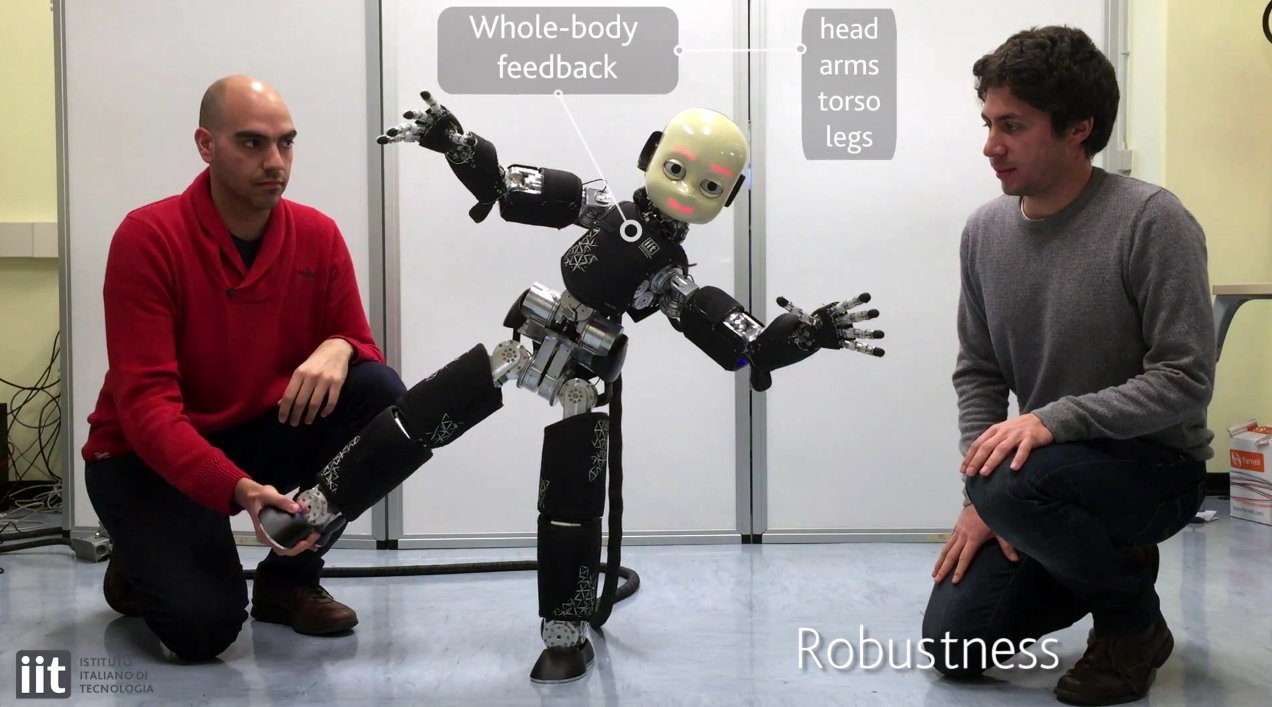
\includegraphics[width=0.65\textwidth]{images/single_foot_balancing.jpg}}
\caption{The picture shows the iCub while performing compliant single foot balancing. Details on the controller can be found in \cite{Nori2015a}. A video of the task is available on youtube\protect\footnotemark.}
\label{fig:footBalancing}
\end{figure}

\footnotetext{\url{https://www.youtube.com/watch?v=SYVCbzGsBF4}.}